\Object{Région}
{
	Les objets \og région\fg assurent la gestion des exclusions mutuelles (\textsl{mutex}), C'est à dire que la tâche utilisant cette région ne sera jamais préemptée, pas même par des tâches de priorité plus haute.

	Les objets de type région peuvent prendre deux états : LIBRE ou OCCUPÉE. À sa création, une région est libre.
}
{
	\begin{itemize}
		\item Identifiant : \lstinline{int} $\in [0, 2^{16} - 1]$
	\end{itemize}
}
{
	Toutes les primitives renvoient -1 en cas d'erreur (\textsl{e.g} plus de mémoire disponible, identifiant invalide, \textsl{etc.}). Sauf indication contraire, elles renvoient 0 en cas de succès.

	\begin{itemize}
		\item \lstinline{int entrer(int id)} : Rentre dans le région dont l'identifiant est passé en paramètre. Dans un contexte monoprocesseur, on est assuré que si la région est déjà occupée, elle l'est par la tâche courante. Dans le cas où la tâche demande à rentrer dans un région dans laquelle elle est déjà, sa demande est ignorée.
		\item \lstinline{int sortir(int id)} : Sort de la région dont l'identifiant est passé en paramètre. Si une tâche demande à sortir d'une région dans laquelle elle n'est pas, sa demande est ignorée.
	\end{itemize}
}
{
\begin{figure} [htp]
\centering
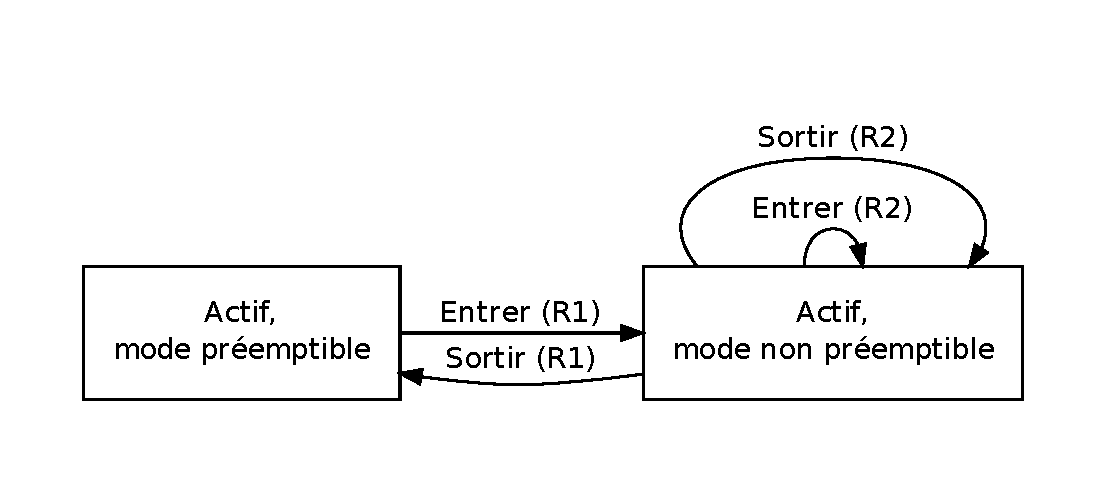
\includegraphics[width=0.6\textwidth]{img/etatRegion.pdf}
\end{figure}
}
{
	Il est à noter que :
	\begin{itemize}
		\item Les opérations d'attente passive et de terminaison de la tâche sont interdites dans une région.
		\item Les régions sont imbricables les unes dans les autres.
		\item Dans un contexte multi-processeur, il peut y avoir concurrence d'accès à la région entre deux tâche. Dans ce cas, la primitive \lstinline{entrer} est bloquante pour la deuxième tâche appelante tant que la région n'est pas libérée.
	\end{itemize}
}
